%document
\documentclass[10pt]{beamer}
%theme
\usetheme{metropolis}
% packages
\usepackage{color}
\usepackage{listings}
\usepackage[ngerman]{babel}
\usepackage[utf8]{inputenc}
\usepackage{multicol}

\usepackage{hyperref}
\hypersetup{colorlinks=true, linkcolor=blue, urlcolor=red}

% color definitions
\definecolor{mygreen}{rgb}{0,0.6,0}
\definecolor{mygray}{rgb}{0.5,0.5,0.5}
\definecolor{mymauve}{rgb}{0.58,0,0.82}

\lstset{
    backgroundcolor=\color{white},
    % choose the background color;
    % you must add \usepackage{color} or \usepackage{xcolor}
    basicstyle=\footnotesize\ttfamily,
    % the size of the fonts that are used for the code
    breakatwhitespace=false,
    % sets if automatic breaks should only happen at whitespace
    breaklines=true,                 % sets automatic line breaking
    captionpos=b,                    % sets the caption-position to bottom
    commentstyle=\color{mygreen},    % comment style
    % deletekeywords={...},
    % if you want to delete keywords from the given language
    extendedchars=true,
    % lets you use non-ASCII characters;
    % for 8-bits encodings only, does not work with UTF-8
    frame=single,                    % adds a frame around the code
    keepspaces=true,
    % keeps spaces in text,
    % useful for keeping indentation of code
    % (possibly needs columns=flexible)
    keywordstyle=\color{blue},       % keyword style
    % morekeywords={*,...},
    % if you want to add more keywords to the set
    numbers=left,
    % where to put the line-numbers; possible values are (none, left, right)
    numbersep=5pt,
    % how far the line-numbers are from the code
    numberstyle=\tiny\color{mygray},
    % the style that is used for the line-numbers
    rulecolor=\color{black},
    % if not set, the frame-color may be changed on line-breaks
    % within not-black text (e.g. comments (green here))
    stepnumber=1,
    % the step between two line-numbers.
    % If it's 1, each line will be numbered
    stringstyle=\color{mymauve},     % string literal style
    tabsize=4,                       % sets default tabsize to 4 spaces
    % show the filename of files included with \lstinputlisting;
    % also try caption instead of title
    language = C,
	showspaces = false,
	showtabs = false,
	showstringspaces = false,
	escapechar = ,
}

\def\ContinueLineNumber{\lstset{firstnumber=last}}
\def\StartLineAt#1{\lstset{firstnumber=#1}}
\let\numberLineAt\StartLineAt



\newcommand{\codeline}[1]{
	\alert{\texttt{#1}}
}

% This Document contains the information about this course.

% Authors of the slides
\author{
    Lecturers:
	%name1
	Mirko Jantschke,
	%name2
	Pascal Scholz
	\\
	%creaters of the slides
	Created by: Richard Mörbitz, Manuel Thieme
}


% Fancy Logo
\titlegraphic{\hfill
\includegraphics[height=1.25cm]{../templates/fsr_logo_cropped}}


\title{Debugging}
\subtitle{Variables}
\date{\today}



% the actual document
\begin{document}

\maketitle

%-------------------------------------------------------------------------------------------------

\begin{frame}{Contents}
	\tableofcontents
\end{frame}

%-------------------------------------------------------------------------------------------------
\section{Einleitung}
%-------------------------------------------------------------------------------------------------

\begin{frame}{It's not a bug...}
	Es gibt verschiede Arten von Bugs:
	\begin{itemize}
		\item Compiletime errors
		\item Runtime errors (\textit{bugs})
	\end{itemize}\ \\\ \\
	\textit{Compiletime errors}: Fehler die beim Compilieren auftreten. K\"onnen relative einfach behoben werden, da der Compiler auf sie hinweist.\\\ \\
	\textit{Bugs}: Treten während der Laufzeit (runtime) des Programms auf. Sie sind schwer zu finden und könnne schlimme Folgen haben.
\end{frame}

%-------------------------------------------------------------------------------------------------

\begin{frame}{... it's a feature.}
	Mögliche Auslöser von Bugs:
	\begin{itemize}
		\item Over- /underflow von Variablen
		\item Division durch Null 
		\item Unendliche Schleifen / Rekursion
		\item Range excess
		\item Segmentation fault
		\item Dereferenzierung von \textit{NULL pointers}
		\item und viele mehr
	\end{itemize}
\end{frame}

%-------------------------------------------------------------------------------------------------

\begin{frame}{Tools für das Debugging}
	Nützliche und weitverbreitete Tools die zum Debugging eingesetzt werden sind:
	\begin{itemize}
		\item Der Compiler
		\item valgrind
		\item GDB
		\item strace (werden wir nicht ausprobieren, nur Hinweis auf Existenz)
		\item ...und viele mehr
	\end{itemize}
	Im folgenden sollen die Möglichkeiten der genannten Tools kurz angerissen werde.
\end{frame}

%-------------------------------------------------------------------------------------------------
\section{Debugging mit dem Compiler - am Beispiel der GCC}

%-------------------------------------------------------------------------------------------------

\begin{frame}{N\"utzliche Flags des GCC}
	Nützliche und weitverbreitete Tools die zum Debugging eingesetzt werden sind:
	\begin{itemize}
		\item -Wunsed (zeigt ungenutze Variable, gilt als Warnung)
		\item -Wall (zeigt [fast]alle Warnung)
		\item -Werror (behandelt Warnung als Fehler, so dass nicht compiliert wird)
		\item -g (default Debugging Informationen) 
		\item und viele mehr, siehe man gcc
	\end{itemize}
\end{frame}

%-------------------------------------------------------------------------------------------------
\begin{frame}[fragile]{Ein Test am Beispiel}
	Versucht einmal, das Programm der linked list wie folgt zu compilieren:
		\begin{lstlisting}[numbers=none]
$ gcc -Wall -Werror <Dateiname>.c\end{lstlisting}
Wenn ihr den Code nicht mehr habt, kopiert ihn euch \href{https://github.com/scholzp/c-lessons/blob/master/materials/memory_allocation/dynmamicMemeory.c}{hier}.
Die Ausgabe sollte wie folgt aussehen (wenn es eine Warnung gibt):
\\
\bigskip
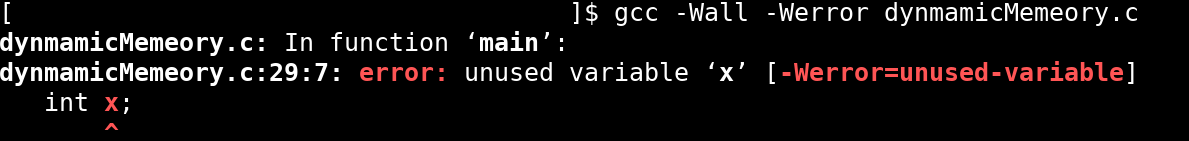
\includegraphics[width = \linewidth]{../img/gccWerror.png}
\end{frame}

%-------------------------------------------------------------------------------------------------
\section{Vorbereitungen für Runtime Debugging}
%-------------------------------------------------------------------------------------------------
\begin{frame}[fragile]{Vorbereitung}
	Normal kompilierten Programmen beinhalten sinnvollerweise keine bzw. wenige Debugginginformationen. Diese blähen die ausführbare Datei auf und bieten zusätzliche Angriffsfläche, da mit ihnen Reverse-Engeneering möglich ist.\\
	\bigskip
	Um Programme mit Debugging-Informationen zu compilieren:
		\begin{lstlisting}[numbers=none]
$ gcc -g <Dateiname>.c\end{lstlisting}
Falls \textit{GDB} noch nicht installiert ist, sollte dies noch getan werden:
		\begin{lstlisting}[numbers=none]
$ sudo pacman -S gdb        #arch
$ sudo apt-get install gdb  #ubuntu\end{lstlisting}

\end{frame}
%-------------------------------------------------------------------------------------------------
\section{Debugging mit GDB}
%-------------------------------------------------------------------------------------------------
\begin{frame}{GDB - Was ist das?}
Der GDB oder GNU Debugger ist ein freies und sehr mächtiges Debugging-Werkzeug. Wenn sich ein Programm nicht wie erwartet verhält, kann man mit ihm dessen Abarbeitung Schritt für Schritt nachvollziehen, um herauszufinden, wo im Quelltext Fehler sein könnte. \\
\bigskip
Generell kann er für alle Fehlerarten (während der Laufzeit) eingesetzt werden. 
\end{frame}

%-------------------------------------------------------------------------------------------------
\begin{frame}{GDB Befehle}
	\begin{itemize}
		\item Wenn gdb ohne ein Programm gestartet wurde kann mit \textbf{file}  \textit{file\_name} eine geladen werden.
		\item Mit \textbf{r[un]} kann das Programm innerhalb von gdb ausgeführt werden.\\
		Als ersten Schritt sollte das Programm so einmal abgearbeitet werden, um genauere Details zum Fehler zu erhalten. Alternativ kann mit \textbf{start} zum Einstiegspunkt (erste Zeile in main) gesprungen werden.
		\item Haltepunkte (Breakpoints) können mit \textbf{b[reak]} \textit{line\_number} oder \textbf{b[reak]} \textit{function\_name} gesetzt werden.\\
		An der vermuteten Stelle des Bugs im Quelltext sollte begonnen werden.
		\item Mit \textbf{p[rint]} \textit{identifier} können Werte angezeigt werden.
		\item \textbf{w[atch]} \textit{identifier} unterbricht das Programm und gibt den Wert von \textit{identifier} aus, sobald diese Variable geändert wird.
	\end{itemize}
\end{frame}

%-------------------------------------------------------------------------------------------------

\begin{frame}{...wenn man den Breakpoint dann einmal erreicht hat.}
	\begin{itemize}
		\item \textbf{n[ext]} f\"uhrt nur die nächste Zeile des Prrgramms aus.
		\item \textbf{s[tep]} f\"urht die nächste Anweisung aus.
		\item Um das Programm bis zum n\"achsten Breakpoint ausführen zu lassen, kann \textbf{c[ontinue]} genutzt werden.
		\item Mit \textbf{backtrace} oder \textbf{bt} k\"onnen die aufgerufenen Funktionen angezeigt werden.\\
		\item Um den Quelltext auszugeben ab eine bestimmten Zeile, kann \textbf{l[ist] Startzeilennummer} genutzt werden.
		\\\ \\
		\item Wenn nur die \textit{Enter-Taste} gedrückt wird, wird der zuletzt eingegebene Befehl ausgeführt.
	\end{itemize}
\end{frame}

%-------------------------------------------------------------------------------------------------

\begin{frame}[fragile]{Bedingte Haltepunkte (breakpoints)}
Nachdem ein Breakpoint gesetzt wurde, wird ihm von GDB eine ID zugewiesen.\\
Diese ID kann genutzt werden, um die Funktionalit\"at von diesem zu erweitern.
	\begin{itemize}
		\item \textbf{con[dition]} \textit{breakpoint\_ID expression} f\"ugt dem Breakpoint eine Bedingung hinzu:
		\begin{lstlisting}[numbers=none,language=bash]
(gdb) br 42
Breakpoint 1 at 0xbada55: file main.c, line 42.
(gdb) condition 1 i@=@@=@3
\end{lstlisting}
		\item Strings m\"ussen definiert werden, bevor sie mit \textbf{strcmp} genutzt werden k\"onnen:
		\begin{lstlisting}
(gdb) br main.c:42
Breakpoint 13 at 0xdeadbeef: file main.c, line 42.
(gdb) set $string_to_compare = "lolwut"
(gdb) cond 13 strcmp ( $stringtocompare, c ) @=@@=@ 0
\end{lstlisting}
	\end{itemize}
\end{frame}

%-------------------------------------------------------------------------------------------------

\begin{frame}{Eine kleine Zusammenfassung}
		\begin{tabular}{|l|l|}
			\hline
			\textbf{file} & L\"adt Programm\\\hline
			\textbf{r[un]} & F\"uhrt ein Programm aus\\\hline
			\textbf{start} & Führt die erste Instruktion eines Programms aus\\\hline
			\textbf{b[reak]} & Setzt einen Breakpoint\\\hline
			\textbf{p[rint]} & Gibt Variable aus\\\hline
			\textbf{w[atch]} & Bei Ver\"anderung unterbreche und gebe Variable aus.\\\hline
			\textbf{n[ext]} & F\"uhre n\"achste Zeile aus und unterbreche\\\hline
			\textbf{s[tep]} & F\"uhre n\"achsten Befehl aus und unterbreche\\\hline
			\textbf{c[ontinue]} & F\"uhrt ein Programm bis zum n\"achsten Breakpoint aus\\\hline
			\textbf{l[ist]} & Gibt Quelltext aus\\\hline
			\textbf{backtrace} / \textbf{bt} & Gibt Aufrufhierarchi der Funktionen aus\\\hline
			\textbf{q[uit]}  & Beendet GDB (und das darin ausgeführte Programm)\\\hline
		\end{tabular}	
\end{frame}
%-------------------------------------------------------------------------------------------------
\begin{frame}{...und ein Beispiel}
Im Beispiel-Programm ist ein kleiner Fehler versteckt. Hier eine Idee, wie man vorgehen könnte:
\begin{itemize}
    \item F\"uhrt das Programm innerhalb von GDB einmal aus, um zu schauen, was der Fehler ist (es passiert nichts, beendet das Programm. Eventuell gibt es einen Hinweis..)
    \item Mit \textbf{s[tep]} kann das Programm schrittweise abgearbeitet werden, wenn man keine Idee hat, wo man anfangen kann. (Bei großen Programmen eventuell unpraktisch)
    \item Hat man eine verdächtige Stelle gefunden, bietet es sich an den Quelltext mit \textbf{l[ist] Startzeilennummer} anzusehen.
    \item Falls nötig entsprechende Variablen und deren Ver\"anderung mit \textbf{p[int] idendifier} ansehen. 
\end{itemize}
EIN HINWEIS: Mit der Tastenkombination \texttt{strg+C} kann man laufende Programme (im Terminal) beenden. \\
Bitte nicht auf die n\"achste Folie schauen, da steht die Lösung.
\end{frame}
%-------------------------------------------------------------------------------------------------

\begin{frame}[fragile]{Die Auflösung}
\begin{lstlisting}
int power(int base, int exponent) {
	int result = 1;
	int count  = 0;
	while(count < exponent) % {
		result *= base;     %  
		++count;            % }
	return result;
}\end{lstlisting}

Wir haben hier eine Endlosschleife. Auf den ersten Blick ist aber alles in Ordnung und sollte funkionieren. Aber warum tut es das nicht? \\
\bigskip
Es fehlen die geschweiften Klammern nach dem while-Statement. Es wird nur result berechnet, nicht aber count inkrementiert.\\
$\rightarrow$  Ein Klammernpaar nach dem while-Statement, das nach Zeile 6 geschlossen wird, löst das Problem.
\end{frame}

%-------------------------------------------------------------------------------------------------
\section{Debugging mit Valgrind}
%-------------------------------------------------------------------------------------------------
\begin{frame}{Was ist Valgrind}
Valgrind ist ein Framwork, welches verschiede Werkzeuge anbietet. Beispielsweise bietet es Werkzeuge um Bugs im Speicher- oder Threadmangemant zu finden. Wir befassen uns nur mit dem Speichertool, mit welchem wir selbst Fehler in Programmen aufdecken k\"onnen, die es nicht zum Absturz bringen.\\
\bigskip
Weitere Informationen zu Valgrind können auf der offiziellen \href{http://valgrind.org/}{Seite} gefunden werden. 
\end{frame}
%-------------------------------------------------------------------------------------------------

\begin{frame}[fragile]{Den Memory check von Valgrind verwenden}
Nachdem das Programm mit Debugginginformationen kompiliert wurde, kann man valgrind starten und das Programm als Argument übergben:
\begin{lstlisting}[numbers=none,language=bash]
$ valgrind <Programmname>\end{lstlisting}
Um weiter Informationen über Memory-Leaks zu erhalten:
\begin{lstlisting}[numbers=none,language=bash]
$ valgrind --leak-check=full <Programmname>\end{lstlisting}
Wenn man nun noch mehr über die Quelle der Leaks erfahren möchte:
\begin{lstlisting}[numbers=none,language=bash]
$valgrind --leak-check=full --track-origins=yes <Prog.-name>\end{lstlisting}

Mehr Informationen zur Verwendung können auf der offiziellen \href{http://valgrind.org/docs/manual/quick-start.html}{Seite} von Valgrind gefunden werden.
\end{frame}
%-------------------------------------------------------------------------------------------------
\begin{frame}[fragile]{Wir probieren es aus...}
Wir haben im letzten Kurs ein Programm mit Speicherbugs geschrieben. Dieses sollten wir eventuell noch fertigstellen, damit ihr ein gutes Beispiel habt. \\
\bigskip
Die Rede ist von der verketteten Liste. Falls ihr den Code nicht mehr habt, findet ihr in \href{https://github.com/scholzp/c-lessons/blob/master/materials/memory_allocation/dynmamicMemeory.c}{hier}.\\
Nun versuchen wir den Fehler zu finden
\end{frame}
%-------------------------------------------------------------------------------------------------
\begin{frame}[fragile]{Möglicher Qutput}
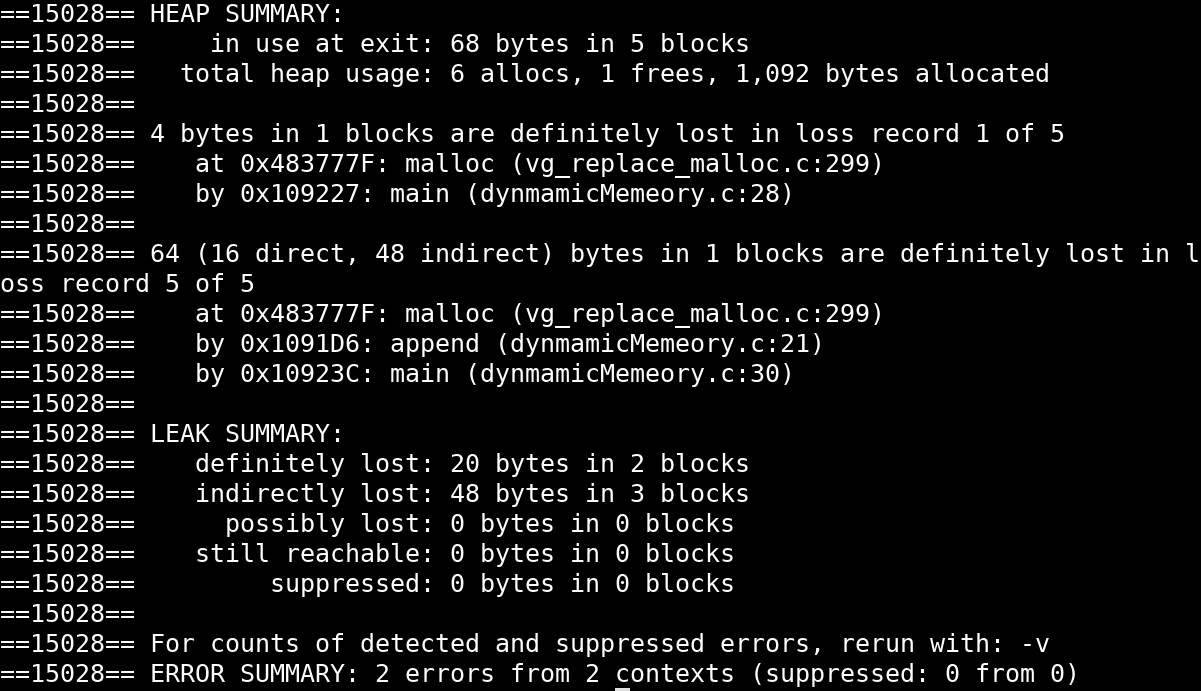
\includegraphics[width = \linewidth]{../img/valgrind.png}
\end{frame}
%-------------------------------------------------------------------------------------------------

\begin{frame}[fragile]{Heap Summary}
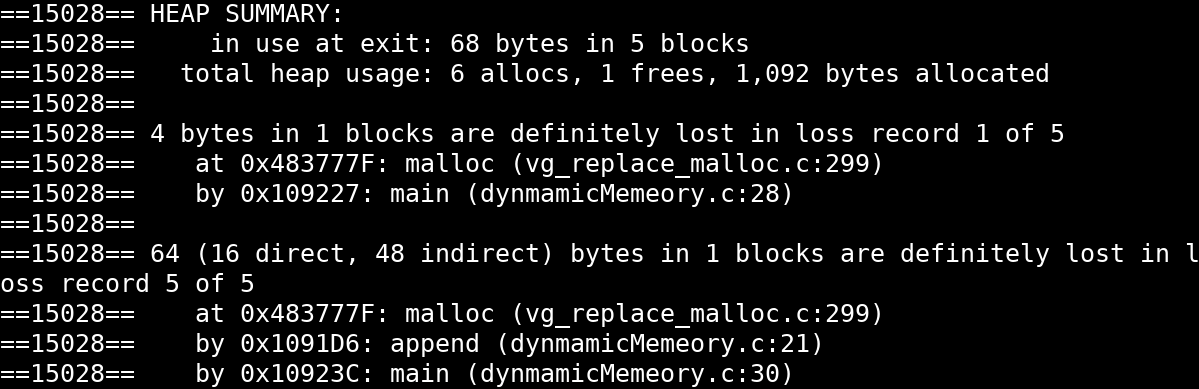
\includegraphics[width = \linewidth]{../img/heapSummary.png}
\begin{itemize}
 \item Statistiken zum Auf dem Heap allokierten Speicher
 \item Backtracing der Funktionsaufrufe in denen Speicher verlorengegangen ist
\end{itemize}

\end{frame}
%-------------------------------------------------------------------------------------------------
\begin{frame}[fragile]{Leak Summary}
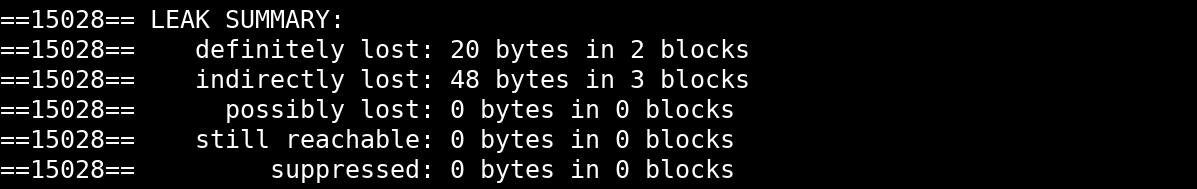
\includegraphics[width = \linewidth]{../img/leakSummary.png}
\begin{itemize}
 \item Ist die zusammenfassende Statistik
 \item definitily lost: Speicher auf den von Pointern direkt gezeigt wurde
 \item indirectly lost: Speicher auf den von Pointer über Pointer indirekt gezeigt wurde.
 \item Im Falle von Fehlern durch das Verwenden von uninitialisierten Variablen wird zusätzlich gewarnt. 
\end{itemize}
Ebenfalls auf der offiziellen Seite wird noch einmal genau erklärt, was die einzelnen Angaben bedeuten.
\end{frame}
%-------------------------------------------------------------------------------------------------
\section{Aufgabe}
%-------------------------------------------------------------------------------------------------
\begin{frame}{Zum Ausprobieren}
Im Beispiel-Programm sind 2 kleine Fehler versteckt, die das Programm zum Absturz bringen. Versucht einmal, diese beiden Fehler mit GDB, valgrind und dem Compiler zu finden. Hier eine Idee, wie man vorgehen könnte:
\begin{itemize}
 \item F\"uhrt das Programm einmal aus, um zu schauen, was der Fehler ist (es sollte abstürzen)
 \item Lasst euch einen Backtrace anzeigen, um die Funktionsaufrufe nachzuvollziehen.
 \item Wenn ihr verstanden habt, was nicht funktionieren könnte, lasst euch den Quelltext anzeigen. (Wenn nicht, meldet euch)
 \item Von hier aus solltet ihr alleine weiter kommen.
\end{itemize}
 Bitte nicht auf die n\"achste Folie schauen, da steht die Lösung. 
\end{frame}
%-------------------------------------------------------------------------------------------------
\begin{frame}[fragile]{Und die Aufl\"osung}
Beide Fehler sind in dieser kleinen Funktion:
\begin{lstlisting}
void a(int n){
  if(n = 0)
    return;
  a(n);
}\end{lstlisting}
In main() wird d(), in d() wird c(), in c() wird b() und in d() wird a() aufgerufen. Die Funktion a() ruft sich selbst rekursiv auf. Sie hat folgende Fehler, die zu einer unendlichen Rekursion und damit wegen ausgehenden Stackspeicher zu einem Absturz f\"uhren:\\
In Zeile 2: Kein Vergleich, sondern Zuweisung. Sollte n == 0. sein\\
In Zeile 4: Kein Dekrementieren um Abbruchbedingungen zu erreichen. Sollte a(n-1) sein.
\end{frame}
%-------------------------------------------------------------------------------------------------
\begin{frame}[fragile]{Und die Aufl\"osung}
Beide Fehler sind in dieser kleinen Funktion:
\begin{lstlisting}
void a(int n){
  if(n = 0)
    return;
  a(n);
}\end{lstlisting}
In main() wird d(), in d() wird c(), in c() wird b() und in d() wird a() aufgerufen. Die Funktion a() ruft sich selbst rekursiv auf. Sie hat folgende Fehler, die zu einer unendlichen Rekursion und damit wegen ausgehenden Stackspeicher zu einem Absturz f\"uhren:\\
In Zeile 2: Kein Vergleich, sondern Zuweisung. Sollte n == 0. sein\\
In Zeile 4: Kein Dekrementieren um Abbruchbedingungen zu erreichen. Sollte a(n-1) sein.
\end{frame}
%-------------------------------------------------------------------------------------------------
\begin{frame}[fragile]{Noch mehr Bugs...}
Im Ordner \href{https://github.com/scholzp/c-lessons/tree/master/materials}{Materials} in diesem Repository befindet sich Ordner 1\_* bis 6\_* (* ist eine Wildcard) mit verbuggtem Code. \\
\bigskip
Viel Erfolg...
\end{frame}
%-------------------------------------------------------------------------------------------------

\end{document}
